\scanpage{35}
% Long diagonal strokes cancel this sheet.
\deleted{reference [1] for expose X :}

\deleted{[1] J. Ax , Some conjectures of Serre on cohomological dime\deleted{\unsure{s|a|n}}nsion, Proc. Amer. Math. Soc. 16 (1965) 1214-1221 .}
\figure{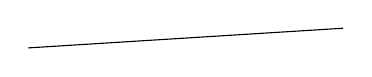
\begin{tikzpicture}\draw (0,0)--(4,0.25);\end{tikzpicture}}

\deleted{exp X p. 7 here is what is to be added:}

\deleted{Le corps residuel de $R'$ est $k$ puisque nous avons suppose $\bar{G}$ un \deleted{$\unsure{p|m}$} $\handwritten{\ell}$-groups, donc que les racines $\handwritten{\ell}$-iemes de 1 so\deleted{\unsure{t|n}}nt dans $K$. On a un diagramme}
\diagram{\begin{tikzcd}[ampersand replacement=\&]
\deleted{H'} \handwritten{\arrow[r,hook]}\handwritten{\arrow[d,hook]} \& \deleted{G'} \handwritten{\arrow[r]}\handwritten{\arrow[d,hook]} \& \deleted{\bar{G}} \handwritten{\arrow[d,equal]} \\
\deleted{H} \handwritten{\arrow[r,hook]} \& \deleted{G} \handwritten{\arrow[r]} \& \deleted{\bar{G}}\rlap{,}
\end{tikzcd}}
\figure{\begin{tikzpicture}\draw (0,0)--(3.2,0);\end{tikzpicture}}

\deleted{exp XII, 5.10: A reference for my paper on alg.approx is}

\deleted{M. Artin, Algebraic approximation of structures over complete local rings, (a paraitre).}

\deleted{\handwritten{(}The explicit result is Theorem (3.1)\handwritten{)}.}
\figure{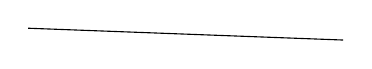
\begin{tikzpicture}\draw (0,0)--(4,-0.15);\end{tikzpicture}}

\deleted{exp IX p.\handwritten{34} here are some references:}

\deleted{A. Douady, Cohomologie des groupes compacts totalement discontinus, Séminaire Bourbaki, exposé 189, (th\handwritten{\unsure{ê|é}}or\handwritten{è}me 4.3)}

\deleted{S. Lang, Rapport sur la cohomologies des groupes, Benjamin 1966. (th\handwritten{é}or\handwritten{è}me 12, p.207).}

\deleted{Ch.C. Tsen, Divisionsalgebren über Funktionen\deleted{\unsure{f|k}}körper, Nachr. Ges. Wiss. Göttingen (1933) \handwritten{335-339} .}
% archive sheet number: 34
